% res_model.tex  -- written by Abhijeet
\subsection{Latency and Throughput Model}
Counting states gives a start-to-done latency of $3N$ cycles: 1
\textsc{Clear}, $N$ \textsc{Feed}, $2N-2$ \textsc{Drain} and 1
\textsc{Done}. With back-to-back starts the period is also $3N$, so the
throughput is $N^3/3N = N^2/3$ MACs per cycle. Table~\ref{tab:model}
compares this model with measurements; latency matches exactly for every
$N$. The small excess in the period comes from filling and emptying the
pipeline over a 50-product run. Fig.~\ref{fig:scaling} shows that the
systolic period grows linearly while the sequential baseline grows as
$N^3$.

\begin{table}[t]
\centering
\caption{Analytical model vs.\ measured cycles}
\label{tab:model}
\setlength{\tabcolsep}{3pt}
\begin{tabular}{@{}lrrrr@{}}
\toprule
$N$ & \textbf{latency} & \textbf{model} & \textbf{period (meas.)} & \textbf{MAC/cycle}\\
\midrule
2  & 6  & 6  & 6.14  & 1.30 \\
3  & 9  & 9  & 9.20  & 2.93 \\
4  & 12 & 12 & 12.26 & 5.22 \\
8  & 24 & 24 & 24.50 & 20.89 \\
16 & 48 & 48 & 48.98 & 83.62 \\
\midrule
\multicolumn{5}{@{}l}{Tiled GEMM on 4$\times$4: 8$\times$8 model 105 / meas.\ 105; 12$\times$12: 319 / 319}\\
\multicolumn{5}{@{}l}{WS, $M$ rows of $A$: $M$=4 model 15 / meas.\ 15; $M$=16: 27 / 27}\\
\bottomrule
\end{tabular}
\end{table}

\begin{figure}[t]
\centering
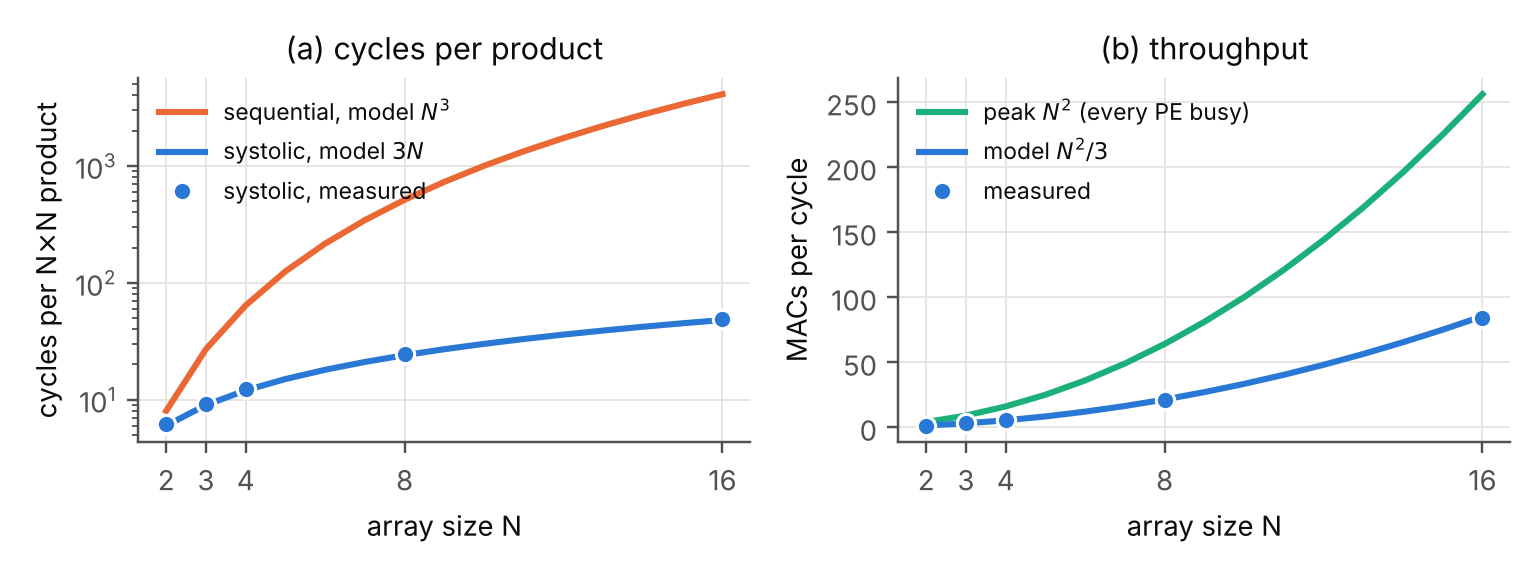
\includegraphics[width=\columnwidth]{fig_scaling.png}
\caption{Array-size sweep: (a) cycles per $N\times N$ product, (b) throughput vs.\ the peak of $N^2$ MACs/cycle.}
\label{fig:scaling}
\end{figure}

The PE utilisation of the OS design is fixed at
$N^3/(N^2\cdot 3N) = 1/3$, independent of $N$
(Fig.~\ref{fig:scaling}b). The wavefront needs $N-1$ cycles to reach the
far corner of the array and $N-1$ cycles to leave it, and the accumulators
must be emptied before the next product, so PEs are idle during both ramps.
